% A good introduction to latex can be found here:
%    http://www.cse.ohio-state.edu/~hank/latex/lshort141.pdf

\documentclass[9.5pt]{extarticle}

\usepackage{full page}  % make the margins somewhat smaller than the default
\usepackage{graphicx}
\usepackage{amsmath}
\usepackage{indentfirst}
\usepackage{color}
\usepackage{cite}
\usepackage{wasysym}
\usepackage{amssymb}
\usepackage{multirow}
\usepackage{float}
\usepackage{lscape}
\usepackage{alltt} 
\usepackage{listings}
\usepackage{booktabs}
\usepackage{mathtools}
\usepackage{fancyhdr}
\usepackage[table,xcdraw]{xcolor}

\DeclarePairedDelimiter{\ceil}{\lceil}{\rceil}
\DeclarePairedDelimiter{\floor}{\lfloor}{\rfloor}

\definecolor{dkgreen}{rgb}{0,0.6,0}
\definecolor{gray}{rgb}{0.5,0.5,0.5}
\definecolor{mauve}{rgb}{0.58,0,0.82}


\usepackage{listings}  %  needed for source code listings

\lstset{frame=tb,
  language= java,
  aboveskip=1.5mm,
  belowskip=1.5mm,
  showstringspaces=false,
  columns=flexible,
  basicstyle={\small\ttfamily},
  keywordstyle=\color{blue},
  commentstyle=\color{dkgreen},
  stringstyle=\color{mauve},
  breaklines=true,
  tabsize=2,
  numbers=left,
  stepnumber=1,    
  firstnumber=1,
  numberfirstline=true
}
       

% set the document title, author, and date here.
%  once set, the \maketitle command (within the document)
%  will display them nicely
\title{Probabilistic Reasoning Assignment}
\author{Chua Zheng Fu Edrei}

\begin{document}
\maketitle

\section{Introduction}

In this report, I will present on a hidden markov model representation of the blind robot problem and present a filtering (forward and forward-backward smoothing) method to compute the probability distribution over location that the robot might be in. I will also present the experimental results and discuss the effectiveness of the forward and forward-backward smoothing method. I will also present evidence to demonstrate that a better estimate of state distribution at time steps other than the first or last time step can be computed by using a forward-backward algorithm. Finally, I will discuss a recent paper by Krogh et al. that explains how we can predict the topology of protein using a hidden markov model.


\section{Implementation}

\subsection{Problem statement}
In the given problem, a robot is in a 4x4 maze. The robot can move in four direction (north, south, east, west) but will not move (remain in the same location) it it ran into a wall. The robot has an initial location and does not know either its initial location or how it moved, although it does know that it only makes one move per time step. The robot has a sensor that is able to detect the color of the empty square of the maze it is occupying with an uncertainty error. The floor is painted with one of four colors: red, green, yellow, or blue. The probability that the sensor detects a correct color is 0.88 and the probability that it detects a wrong color is uniformly distributed among the three remaining colors (0.04 each).

\subsection{Model and preprocessing}

We build a state transition model using matrix representation. States are defined as the set of empty squares in the maze and at the beginning, there is an equal probability distribution across all states ($\frac{1}{4}$ for 4 empty squares for instance). The transition can be represented as a transition matrix $T$ similar to the one described in p.579 of the book, in which the entry $T_{ij}$ describes the probability of a transition from state $i$ to $j$. The function for building a transition matrix is given in Listing 1. The basic idea is that each direction (north, south, east, west) has a 0.25 probability of occuring and staying in the same location has a 0 probability of occuring if there are no walls around it. If there is a wall, the probability of going in that direction becomes zero while the probability of staying in the same location increases by 0.25 (we can see it as bouncing off the wall). \verb`findNeighbors` is a function to find the neighboring location (including the same location) (refer to java file for details of implementation). Note that \verb`Matrix` is a class that include a \verb`double[][[]` array and has methods to facilitate the calculation of transpose and the multiplication with another vector (refer to Matrix.java for details of implementation).\\

The sensor model can also be represented as a diagonal matrix $O$ as described in p.579 of the book. The function for building the sensor matrix (four matrices for each color) is given in Listing 2. The basic idea is this: all entries except those along the diagonal are zero. The entry $O_{ii} = rightColor$ if state $i$ is the right color and $O_{ii} = wrondColor$ if state $i$ is the wrong color. The \verb`rightColor` and  \verb`wrongColor` are constants with values of 0.88 and 0.04 respectively.

\begin{lstlisting}[language=java,caption={buildTransition}]
	public void buildTransition(){
        transition = new Matrix(maze.numStates,maze.numStates);
        for(int r = 0; r < maze.height; r++){
            for(int c = 0; c < maze.width; c++){
                int stateNum = maze.getStates(r,c);
                
                if(stateNum == -1) // default zero if it is a wall
                    continue;
                    
                int numWalls;
                List<Integer> neighbors = findNeighbors(r,c);

                if(neighbors.size()==1) {
                    transition.data[stateNum][stateNum] = 1;
                }else {
                    numWalls = 5 - neighbors.size();
                    transition.data[stateNum][stateNum] = (double)numWalls/4.0;
                    for(int num: neighbors){
                        if(num == stateNum) continue;
                        transition.data[stateNum][num] = 0.25; // 0.25 probability for each direction
                    }
                }
            }
        }
        transitionTranspose = transition.transpose();
    }
\end{lstlisting}

\begin{lstlisting}[language=java,caption={buildSensor}]
	public void buildSensor(){
        // initialise the four different sensor matrices
        sensorRed = new Matrix(maze.numStates,maze.numStates);
        // .. do the same as above for sensorGreen, sensorBlue and sensorYellow
        for(int r = 0; r < maze.height; r++){
            for(int c = 0; c < maze.width; c++){
                int stateNum = maze.getStates(r,c);
                // skip if it is a wall
                if(stateNum == -1)
                    continue;
                // Set the diagonal of the sensor matrices to its respective probability
                sensorRed.data[stateNum][stateNum] = wrongColor;
                 // .. do the same for sensorGreen, sensorBlue and sensorYellow
                switch (maze.getChar(r,c)){
                    case 'r': sensorRed.data[stateNum][stateNum] = rightColor;
                        break;
                     // .. do the same as above for sensorGreen, sensorBlue and sensorYellow
                    default:
                        break;
                }
            }
        }
    }
\end{lstlisting}

\subsection{Forward method}

Using the forward method, we can calculate a vector that represents the probability distribution across all states using a the matrix equation given: $f_{1:t+1} = \alpha O_{t+1}T^{T}f_{1:t}$, where $f$ is the vector of probability distribution across states, $\alpha$ is the normalization constant, $O_{t+1}$ is the sensor matrix (for the color observed in time step $t+1$ and $T^T$ is the transposition of the transition matrix. We take the transpose because we are interested in reach a state instead of getting from a state (as that is the guiding principle for constructing the transition matrix). The proof for the correctness of this formulation is described in p.572 of the book and it make use of Baye's rule and the Markov assumption. Listing 3 gives the implementation of the forward method, multiplying the vector at each time step with the respective matrices in the correct sequence. We loop through all the time steps so we can keep the probability distribution at each time step (if we are only interested in the distribution for the final step, we can just keep the previous vector $f$ since the recursive definition requires knowledge of the distribution one step before). Note that \verb`normalize` is a function that normalizes a vector such that the sum of all the values in the vector adds up to 1. The implementation for \verb`normalize` is straightforward and the interested reader can refer to the java file for details.

\begin{lstlisting}[language=java,caption={forward}]
	public void forward(){
        for(int t = 1; t < numSteps; t++){
            // multiply with the transpose of the transition matrix
            vectors[t] = transitionTranspose.multiplyVector(vectors[t-1]);
            switch (sensorData[t]){ // multiply with the corresponding sensor matrix
                case 'r': vectors[t] = sensorRed.multiplyVector(vectors[t]); break;
                case 'b': vectors[t] = sensorBlue.multiplyVector(vectors[t]); break;
                case 'g': vectors[t] = sensorGreen.multiplyVector(vectors[t]); break;
                case 'y': vectors[t] = sensorYellow.multiplyVector(vectors[t]); break;
                default: break;
            }
            normalize(vectors[t]);
        }
    }
\end{lstlisting}

\subsection{Forward-backward smoothing method}

The basic idea of the forward-backward smoothing method is that we can obtain a more accurate probability distribution if we consider the distribution of past states based on knoweldge of future observations. In order to do this, we need to propagte backward (in almost a similar way as described by the forward method) using the matrix equation $b_{k+1:t} = TO_{k+1}b_{k+2:t}$. The implementation for backward propagation is given in Listing 5. Forward-backward smoothing combine the results from forward and backward propagation by multiplying the resultant vector in a point-wise manner and the implementation is given in Listing 4. 


\begin{lstlisting}[language=java,caption={forwardBackward}]
    public void forwardBackward(){
        forward(); // perform forward propagation first
        double[] b = new double[maze.numStates];
        Arrays.fill(b,1);  // initialise backward vector
        for(int t = numSteps-1; t>=1; t--){ // fill in forward backward vector
            fbvectors[t] = pointMultiplyVect(vectors[t],b); // multiply both vectors pointwise
            normalize(fbvectors[t]); // normalize vectors
            b = backward(b,t-1);
        }
    }
\end{lstlisting}

\begin{lstlisting}[language=java,caption={backward}]
    public double[] backward(double[] b, int t){
        double[] result = new double[b.length];
        switch (sensorData[t]){ // multiply with the corresponding sensor matrix
            case 'r': result = sensorRed.multiplyVector(b); break;
            case 'b': result = sensorBlue.multiplyVector(b); break;
            case 'g': result = sensorGreen.multiplyVector(b); break;
            case 'y': result = sensorYellow.multiplyVector(b); break;
            default: break;
        }
        return transition.multiplyVector(result); // multiply with the transition matrix
    }
\end{lstlisting}

\section{Results and Discussion}

In this section, we will present the results obtained from the forward method and the forward-backward smoothing method on a 2x2 maze (simple.maz) and a 4x4 maze (medium.maz). A driver MazeDriver.java is used to simulate the detection of color using the sensor and to present the probability distribution using ascii art. The input is the maze file, the starting position and a sequence of direction eg \{n,n,s,e,w,w\}. The function \verb`getPathFromDirection` in the driver file finds the actual location of the robot at each time step given the starting position and the sequence of directions.\verb`constructSensorData` simulate the role of the sensor by returning a sequence of colors observed using a weighted random number generator (0.88 chance of returning the actual color and 0.04 chance for each remaining color). \verb`drawAscii` present the result using ascii art. All the functions are relatively straightforward to implement and the interested reader is encouraged to look at MazeDriver.java for details.

\begin{figure}[H]
\centering
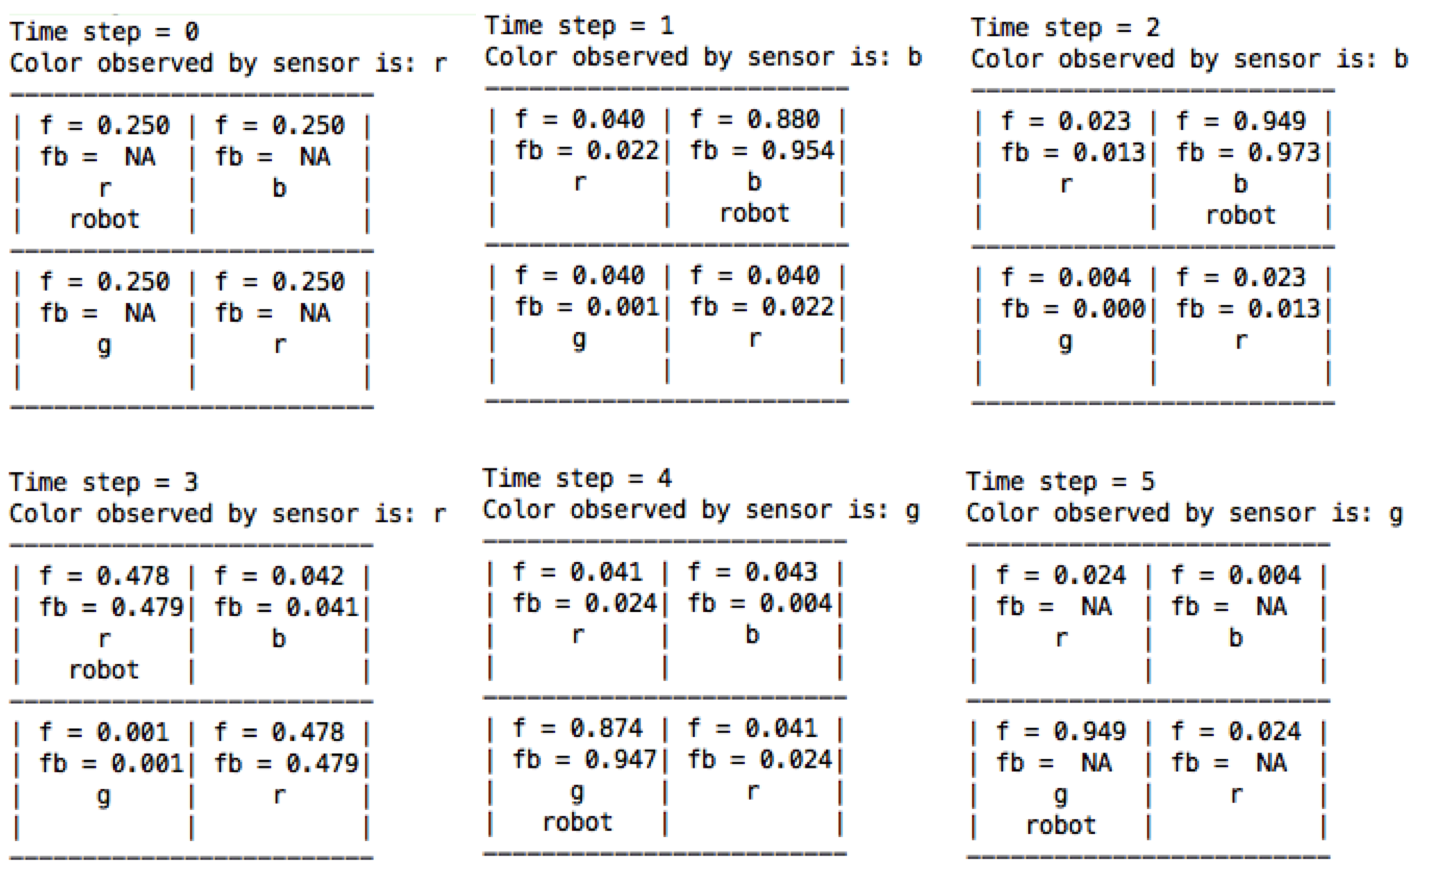
\includegraphics[scale=0.63]{simpleresult.png}
\caption{Probability distribution of simple.maz (f denotes forward propagation and fb denotes forward-backward propagation) when sensor data matches actual data}
\label{Figure 1}
\end{figure}

\begin{figure}[H]
\centering
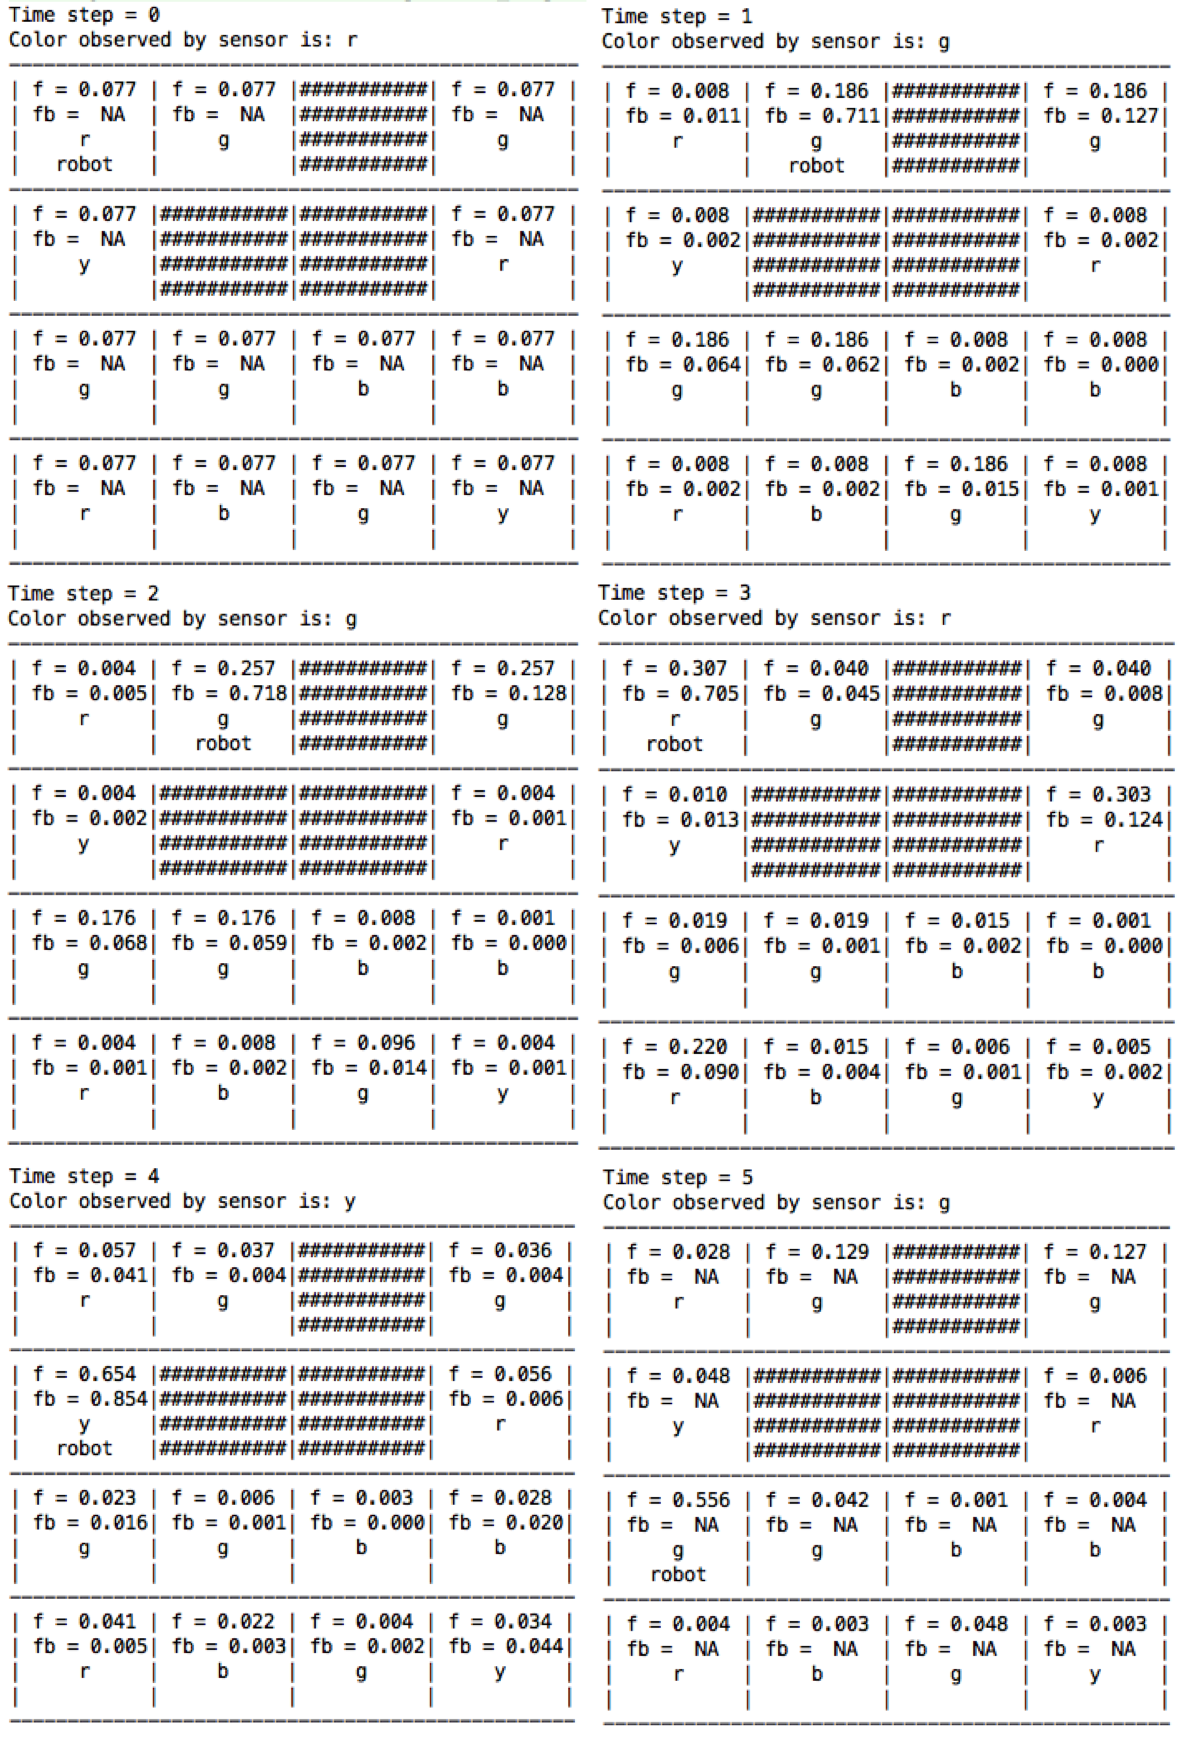
\includegraphics[scale=0.72]{mediumresult2.png}
\caption{Probability distribution of medium.maz (f denotes forward propagation and fb denotes forward-backward propagation) when sensor data matches actual data}
\label{Figure 2}
\end{figure}

\begin{figure}[H]
\centering
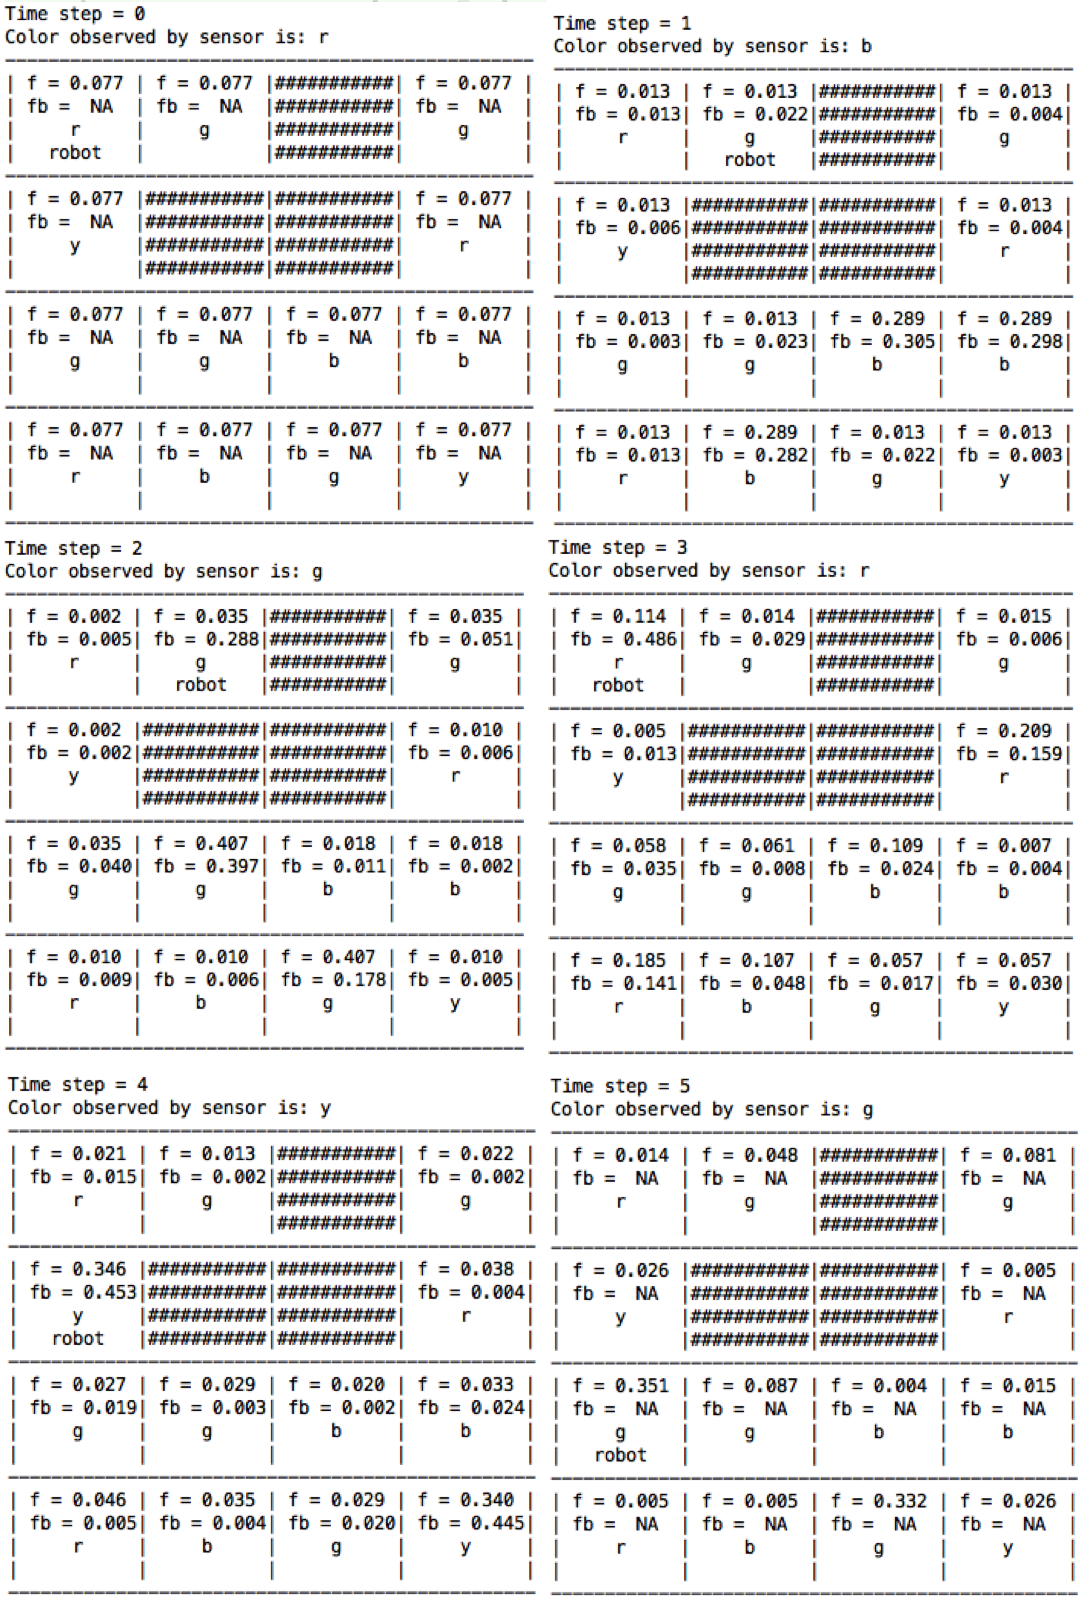
\includegraphics[scale=0.78]{mediumresult.png}
\caption{Probability distribution of medium.maz (f denotes forward propagation and fb denotes forward-backward propagation) when one of the sensor data does not match the actual data}
\label{Figure 3}
\end{figure}

Figure 1 gives the probability distribution of simple.maz and Figure 2 gives the distribution for medium.maz. In both experiments, the sensor data (as given by the weighted randomized function \verb`constructSensorData`) happen to match the actual color data. Figure 3 gives the distribution for medium.maz except that in this case, one of the sensor data gives the wrong value (at time step 1).\\

Note that $f$ (first line of the grid) denotes the probability that the robot is at the given location using the forward method, $fb$ (second line of the grid) denotes the same probability obtained using the forward-backward smoothing method, the third line of the grid gives the actual color of the grid, and \textit{robot} in the fourth line denotes that the robot is currently in that location. The time step and sensor data information is given at the heading of each maze.\\

It is obvious that the probability distribution make sense since the actual location at which the robot is located has a higher probability than the other locations (there are a few exceptions in Figure 3 where the sensor data returns the wrong value, but it is corrected eventually with the progression of time). In addition, we also note that the forward-backward smoothing method almost aways return a more accurate probability distrubution than the forward method, which make sense since it takes into account future observations when constructing the probability distribution of a future step. \\

Table 1, 2 and 3 presents the information in Figure 1, 2 and 3 in a more helpful form for the user. The number given in the table is the probability generated of the robot being in the actual location. Again, we observed that the forward-backward smoothing method return a higher probability in the state that represent the actual location of the robot compared to the forward method. We also note that the improvement accrued by the forward-backward smoothing method is more significant for larger and more complicated mazes (the algorithm yields an average improvement of around 5\% for simple.maz but over a 100\% for medium.maz. In addition, it is interesting that the results using the forward-backward method is less sensitive to wrong sensor information (more robust in that sense) compared to the forward method.


\begin{table}[H]
\resizebox{\textwidth}{!}{%
\begin{tabular}{@{}rcccccc@{}}
\toprule
Time step        & 0    & 1      & 2      & 3      & 4      & 5     \\ \midrule
forward          & 0.25 & 0.88   & 0.949  & 0.478  & 0.874  & 0.949 \\
forward-backward & NA   & 0.954  & 0.973  & 0.479  & 0.947  & NA    \\
Improvement      & NA   & 8.41\% & 2.53\% & 0.21\% & 8.35\% & NA    \\ \bottomrule
\end{tabular}
}
\centering
\caption{Experiements performed to measure improvement in probability distribution using the forward-backward smoothing method for simple.maz (with all sensor data being correct). The number given is the probability generated of the robot being in the actual location}
\label{my-label}
\end{table}

\begin{table}[H]
\resizebox{\textwidth}{!}{%
\begin{tabular}{@{}rcccccc@{}}
\toprule
Time step        & 0     & 1        & 2        & 3        & 4       & 5     \\ \midrule
forward          & 0.077 & 0.186    & 0.257    & 0.307    & 0.654   & 0.556 \\
forward-backward & NA    & 0.711    & 0.718    & 0.705    & 0.854   & NA    \\
Improvement      & NA    & 282.26\% & 179.38\% & 129.64\% & 30.58\% & NA    \\ \bottomrule
\end{tabular}
}
\centering
\caption{Experiements performed to measure improvement in probability distribution using the forward-backward smoothing method for medium.maz (with all sensor data being correct). The number given is the probability generated of the robot being in the actual location}
\label{my-label}
\end{table}

\begin{table}[H]
\resizebox{\textwidth}{!}{%
\begin{tabular}{@{}rcccccc@{}}
\toprule
Time step        & 0     & 1       & 2        & 3        & 4       & 5     \\ \midrule
forward          & 0.077 & 0.013   & 0.035    & 0.114    & 0.346   & 0.351 \\
forward-backward & NA    & 0.022   & 0.288    & 0.486    & 0.453   & NA    \\
Improvement      & NA    & 69.23\% & 722.86\% & 326.32\% & 30.92\% & NA    \\ \bottomrule
\end{tabular}
}
\centering
\caption{Experiements performed to measure improvement in probability distribution using the forward-backward smoothing method for medium.maz (with one incorrect sensor data). The number given is the probability generated of the robot being in the actual location}
\label{my-label}
\end{table}


\section{Literature Review}

I review the article by Anders Krogh,Bjorn Larsson,Gunnar von Heijne and Erik L. L. Sonnhammer titled ``Predicting Transmembrane Protein Topology with a Hidden Markov Model: Application to
Complete Genomes'' (Krogh A., Larsson B., Heijne G.., Sonnhammer E., 2001, Journal of Molecular Biology, 305-3: 567 - 580). This article is interesting because it demonstrates an application of the hidden markov model in bioinformatics (or more specifically, in the protein topology problem which is a subset of the protein folding problem).\\

Krogh et al. demonstrated that with the TMHMM model (based on hidden markov model), they are able to predict 97-98\% of the transmembrane helices (the structure of the orientation in the secondary structure). In addition, the model is able to distiguish between soluble and membrane proteins with both speci®city and sensitivity better than 99\%.\\

The basic idea uses a hidden markov model with hydrophobicity, charge bias, helix lengths etc incorporated as states. The primary HMM parameters are the probabilities of the 20 amino acid residues in the states and the probabilities that determine the length distributions of transmembrane helices. There are two crucial steps involved: training and prediction. The training step estimate the probability distribution associated with the length distributions of transmembrane helices from a set of 160 proteins in The Protein Bank which the locations of the transmembrane helices are known. The prediction step uses the N-best algorithm, which is a modification of the forward-backward smoothing algorithm described in this assignment.\\

I find this article to be helpful because it relates to many of the concepts that we discuss in class. It is also interesting to see how the hidden markov model and the forward-backward smoothing method is applied in recent research.\\


\section{Conclusion}

In this report, I have presented a hidden markov model representation of the blind robot problem and also a filtering (forward and forward-backward smoothing) method to compute the probability distribution over location that the robot might be in. Experimental results revealed that the forward-backward smoothing method is superior to the forward method as it is able to give a more accurate probability distribution. In addition, it has the advantage of being more robust (probability distribution is less affected by wrong sensor information). Finally, I reviewed an article by Krogh et al. that shows how the hidden markov model and a modified version of the forward-backward smoothing algorithm is applied in recent research on the protein topology problem.




\end{document}